\hypertarget{a00373}{}\section{Host Support}
\label{a00373}\index{Host Support@{Host Support}}
Supported features in each A\+A\+X host. 

 \hypertarget{a00373_hostsupport}{}\subsection{Host Support}\label{a00373_hostsupport}
 These tables list A\+A\+X host support for various A\+A\+X interfaces, as well as support for general features. The tables include the version number for the earliest version of each Avid host software which supports the given interface or feature.

The earliest version of each host to support A\+A\+X plug-\/ins is\+: \begin{DoxyItemize}
\item \hyperlink{a00360}{Pro Tools} 10.\+0 \item \hyperlink{a00361}{Media Composer} 8.\+1 \item \hyperlink{a00377}{V\+E\+N\+U\+E} 4.\+1\end{DoxyItemize}
For more information about versioning in A\+A\+X, including how to check for host support of a particular interface, see \hyperlink{a00357}{The Avid Component Framework (A\+C\+F)}.

\hypertarget{a00373_hostsupport_constraints}{}\subsubsection{Platform Support}\label{a00373_hostsupport_constraints}
 \begin{TabularC}{5}
\hline
&{\bf \hyperlink{a00360}{Pro Tools} }&{\bf \hyperlink{a00361}{Media Composer} }&{\bf \hyperlink{a00377}{V\+E\+N\+U\+E} }&

\\\cline{1-5}
\hyperlink{a00283_a6571f4e41a5dd06e4067249228e2249ea89ca3dd6e96895cda14976c1b1ceb826}{A\+A\+X Native} &10.\+0 &8.\+1 &{\itshape none} &\\\cline{1-5}
\hyperlink{a00283_a6571f4e41a5dd06e4067249228e2249ea75f174df4efbeca86eaada126c1d9214}{A\+A\+X D\+S\+P} &10.\+0 &{\itshape none} &4.\+1 &\\\cline{1-5}
\hyperlink{a00335}{A\+A\+X Hybrid} &11.\+0\textsuperscript{$\ast$} &{\itshape none} &{\itshape none} &\\\cline{1-5}
\hyperlink{a00283_a6571f4e41a5dd06e4067249228e2249ead3344696b8298a8b254add3d039ea927}{Offline processing (Audio\+Suite)} &10.\+0 &8.\+1\textsuperscript{$\ast$$\ast$} &{\itshape none} &\\\cline{1-5}
\hyperlink{a00206_a0c5d795c1fd021c5b9b541febc34601aa027df08c137702400a92719828bea44b}{{\ttfamily Process\+Proc} / data model co-\/location} &10.\+0 &8.\+1 &{\itshape none} &\\\cline{1-5}
\hyperlink{a00206_a714f56a9b0ab98a3a5365760adf77624a5f6fe83329b40c9fd0f70fb7b7377121}{{\ttfamily Monolithic} topology} &10.\+0 &8.\+1 &{\itshape none} &\\\cline{1-5}
Native processor architecture &10\+: x86/i386~\newline
11+\+: x86-\/64 &8.\+1+\+: x86-\/64 &4.\+1\+: x86/i386~\newline
4.\+5+\+: x86-\/64 &

\\\cline{1-5}
\end{TabularC}


\begin{DoxyNote}{Note}
Pro Tools 11.\+0 supports A\+A\+X Hybrid processing for real-\/time plug-\/ins only. Support for Audio\+Suite processing for A\+A\+X Hybrid is supported starting in Pro Tools 11.\+1. 

Media Composer 8.\+5 and higher support both multichannel and mono Audio\+Suite processing. Earlier versions of Media Composer support mono only.
\end{DoxyNote}
\hypertarget{a00373_hostsupport_describe}{}\subsubsection{Describe Interfaces}\label{a00373_hostsupport_describe}
 \begin{TabularC}{5}
\hline
&{\bf \hyperlink{a00360}{Pro Tools} }&{\bf \hyperlink{a00361}{Media Composer} }&{\bf \hyperlink{a00377}{V\+E\+N\+U\+E} }&

\\\cline{1-5}
\hyperlink{a00049}{A\+A\+X\+\_\+\+I\+A\+C\+F\+Collection} &10.\+0 &8.\+1 &4.\+1 &\\\cline{1-5}
\hyperlink{a00050}{A\+A\+X\+\_\+\+I\+A\+C\+F\+Component\+Descriptor} &10.\+0 &8.\+1 &4.\+1 &\\\cline{1-5}
~~~~~~~~\hyperlink{a00051}{V2} &11.\+0 &8.\+1 &4.\+5? &\\\cline{1-5}
~~~~~~~~\hyperlink{a00052}{V3} &12.\+8 &{\itshape none} &5.\+6 &\\\cline{1-5}
\hyperlink{a00057}{A\+A\+X\+\_\+\+I\+A\+C\+F\+Effect\+Descriptor} &10.\+0 &8.\+1 &4.\+1 &\\\cline{1-5}
~~~~~~~~\hyperlink{a00058}{V2} &11.\+0 &8.\+1 &4.\+5? &\\\cline{1-5}
\hyperlink{a00079}{A\+A\+X\+\_\+\+I\+A\+C\+F\+Property\+Map} &10.\+0 &8.\+1 &4.\+1 &\\\cline{1-5}
~~~~~~~~\hyperlink{a00080}{V2} &11.\+0 &8.\+1 &4.\+5? &\\\cline{1-5}
~~~~~~~~\hyperlink{a00081}{V3} &12.\+9 &{\itshape none} &5.\+6 &\\\cline{1-5}
\hyperlink{a00056}{A\+A\+X\+\_\+\+I\+A\+C\+F\+Description\+Host} &12.\+8 &{\itshape none} &{\itshape none} &\\\cline{1-5}
\hyperlink{a00065}{A\+A\+X\+\_\+\+I\+A\+C\+F\+Feature\+Info} &12.\+8 &{\itshape none} &{\itshape none} &\\\cline{1-5}
\end{TabularC}


\hypertarget{a00373_hostsupport_runtime}{}\subsubsection{Run-\/\+Time Interfaces}\label{a00373_hostsupport_runtime}
 \begin{TabularC}{5}
\hline
&{\bf \hyperlink{a00360}{Pro Tools} }&{\bf \hyperlink{a00361}{Media Composer} }&{\bf \hyperlink{a00377}{V\+E\+N\+U\+E} }&

\\\cline{1-5}
\hyperlink{a00048}{A\+A\+X\+\_\+\+I\+A\+C\+F\+Automation\+Delegate} &10.\+0 &8.\+1 &4.\+1 &\\\cline{1-5}
\hyperlink{a00053}{A\+A\+X\+\_\+\+I\+A\+C\+F\+Controller} &10.\+0 &8.\+1 &4.\+1 &\\\cline{1-5}
~~~~~~~~\hyperlink{a00054}{V2} &11.\+0 &8.\+1 &{\itshape none} &\\\cline{1-5}
~~~~~~~~\hyperlink{a00055}{V3} &12.\+4 &8.\+6 &{\itshape none} &\\\cline{1-5}
\hyperlink{a00059}{A\+A\+X\+\_\+\+I\+A\+C\+F\+Effect\+Direct\+Data} &10.\+0 &8.\+1 &4.\+1 &\\\cline{1-5}
\hyperlink{a00060}{A\+A\+X\+\_\+\+I\+A\+C\+F\+Effect\+G\+U\+I} &10.\+0 &8.\+1 &4.\+1 &\\\cline{1-5}
\hyperlink{a00061}{A\+A\+X\+\_\+\+I\+A\+C\+F\+Effect\+Parameters} &10.\+0 &8.\+1 &4.\+1 &\\\cline{1-5}
~~~~~~~~\hyperlink{a00062}{V2} &11.\+0 &8.\+1 &4.\+5? &\\\cline{1-5}
~~~~~~~~\hyperlink{a00063}{V3} &11.\+2 &8.\+1 &{\itshape none} &\\\cline{1-5}
~~~~~~~~\hyperlink{a00064}{V4} &{\itshape none} &{\itshape none} &5.\+6 &\\\cline{1-5}
\hyperlink{a00066}{A\+A\+X\+\_\+\+I\+A\+C\+F\+Host\+Processor} &10.\+0 &8.\+1 &{\itshape none} &\\\cline{1-5}
~~~~~~~~\hyperlink{a00067}{V2} &12.\+0 &{\itshape none} &{\itshape none} &\\\cline{1-5}
\hyperlink{a00068}{A\+A\+X\+\_\+\+I\+A\+C\+F\+Host\+Processor\+Delegate} &10.\+0 &{\itshape none} &{\itshape none} &\\\cline{1-5}
~~~~~~~~\hyperlink{a00069}{V2} &11.\+0 &{\itshape none} &{\itshape none} &\\\cline{1-5}
~~~~~~~~\hyperlink{a00070}{V3} &12.\+0 &{\itshape none} &{\itshape none} &\\\cline{1-5}
\hyperlink{a00071}{A\+A\+X\+\_\+\+I\+A\+C\+F\+Host\+Services} &10.\+0 &8.\+1 &4.\+1? &\\\cline{1-5}
~~~~~~~~\hyperlink{a00072}{V2} &12.\+0 &8.\+6 &{\itshape none} &\\\cline{1-5}
~~~~~~~~\hyperlink{a00073}{V3} &12.\+8.\+3 &none &{\itshape none} &\\\cline{1-5}
\hyperlink{a00078}{A\+A\+X\+\_\+\+I\+A\+C\+F\+Private\+Data\+Access} &10.\+0 &8.\+1 &4.\+1 &\\\cline{1-5}
\hyperlink{a00082}{A\+A\+X\+\_\+\+I\+A\+C\+F\+Transport} &10.\+0 &8.\+5 (partial) &{\itshape none} &\\\cline{1-5}
~~~~~~~~\hyperlink{a00083}{V2} &10.\+3.\+7 &8.\+5 (partial) &{\itshape none} &\\\cline{1-5}
\hyperlink{a00084}{A\+A\+X\+\_\+\+I\+A\+C\+F\+View\+Container} &10.\+0 &8.\+1 &4.\+1 &\\\cline{1-5}
~~~~~~~~\hyperlink{a00085}{V2} &12.\+0.\+1 &{\itshape none} &{\itshape none} &\\\cline{1-5}
\hyperlink{a00074}{A\+A\+X\+\_\+\+I\+A\+C\+F\+Page\+Table} &12.\+8 &{\itshape none} &5.\+7 &\\\cline{1-5}
~~~~~~~~\hyperlink{a00075}{V2} &12.\+8.\+2 &{\itshape none} &{\itshape 5.\+7} &\\\cline{1-5}
\hyperlink{a00076}{A\+A\+X\+\_\+\+I\+A\+C\+F\+Page\+Table\+Controller} &{\itshape none} &{\itshape none} &5.\+7 &\\\cline{1-5}
\end{TabularC}


\hypertarget{a00373_hostsupport_features}{}\subsubsection{Features}\label{a00373_hostsupport_features}
 \begin{TabularC}{5}
\hline
&{\bf \hyperlink{a00360}{Pro Tools} }&{\bf \hyperlink{a00361}{Media Composer} }&{\bf \hyperlink{a00377}{V\+E\+N\+U\+E} }&

\\\cline{1-5}
\hyperlink{a00206_ad8af5ef008b2bd478add9a0acb0a1d85}{Surround Stem Formats} (3-\/8 channels) &10.\+0 &8.\+1 &{\itshape none} &\\\cline{1-5}
\hyperlink{a00206_ad8af5ef008b2bd478add9a0acb0a1d85a434dbed527c350cb45787299ead28156}{7.1.2 Stem Format} &{\itshape 12.\+8} &{\itshape none} &{\itshape none} &\\\cline{1-5}
\hyperlink{a00206_ad8af5ef008b2bd478add9a0acb0a1d85}{Ambisonics Stem Formats} &{\itshape 12.\+8.\+2} &{\itshape none} &{\itshape none} &\\\cline{1-5}
\hyperlink{a00356}{Plug-\/in type conversion} &10.\+3.\+8, 11.\+0\textsuperscript{$\ast$}, 11.\+1 &{\itshape none} &{\itshape none} &\\\cline{1-5}
\hyperlink{a00339}{Auxiliary Output Stems} &10.\+0 &{\itshape none} &{\itshape none} &\\\cline{1-5}
\hyperlink{a00338}{Sidechain Inputs} &10.\+0 &8.\+5 &{\itshape none} &\\\cline{1-5}
\hyperlink{a00336}{M\+I\+D\+I} &10.\+0 &{\itshape none} &{\itshape none} &\\\cline{1-5}
\hyperlink{a00349}{Automation} recording and playback &10.\+0 &{\itshape none} &{\itshape none} &\\\cline{1-5}
Plug-\/in presets &10.\+0 &8.\+4 &4.\+1 &\\\cline{1-5}
External control surfaces &10.\+0 &8.\+1 &none &\\\cline{1-5}
\end{TabularC}


\hypertarget{a00373_host_compatibility_notes}{}\subsection{Host Compatibility Notes}\label{a00373_host_compatibility_notes}
\begin{DoxySeeAlso}{See also}
\hyperlink{a00360_aax_pro_tools_guide_07_compatibility_notes}{Compatibility Notes} in the \hyperlink{a00360}{Pro Tools Guide} document
\end{DoxySeeAlso}

\begin{DoxyRefList}
\item[\label{a00381__compatibility_notes000023}%
\hypertarget{a00381__compatibility_notes000023}{}%
Member \hyperlink{a00024_ab6fce0aee8fb08695ac8a112b3c3e7fa}{A\+A\+X\+\_\+\+C\+Midi\+Packet\+:\+:m\+Is\+Immediate} ]This value is not currently set. Use {\ttfamily m\+Timestamp == 0} to detect immediate packets  
\item[\label{a00381__compatibility_notes000024}%
\hypertarget{a00381__compatibility_notes000024}{}%
Member \hyperlink{a00033_a37efc08612535de4712bd59445ce8fbf}{A\+A\+X\+\_\+\+C\+Parameter$<$ T $>$\+:\+:A\+A\+X\+\_\+\+C\+Parameter} (A\+A\+X\+\_\+\+C\+Param\+I\+D identifier, const \hyperlink{a00113}{A\+A\+X\+\_\+\+I\+String} \&name, T default\+Value, const A\+A\+X\+\_\+\+I\+Taper\+Delegate$<$ T $>$ \&taper\+Delegate, const A\+A\+X\+\_\+\+I\+Display\+Delegate$<$ T $>$ \&display\+Delegate, bool automatable=false)]As of Pro Tools 10.\+2, D\+A\+E will check for a matching parameter N\+A\+M\+E and not an I\+D when reading in automation data from a session saved with an A\+A\+X plug-\/ins R\+T\+A\+S/\+T\+D\+M counter part. 

As of Pro Tools 11.\+1, A\+A\+E will first try to match I\+D. If that fails, A\+A\+E will fall back to matching by Name. 
\item[\label{a00381__compatibility_notes000005}%
\hypertarget{a00381__compatibility_notes000005}{}%
Module \hyperlink{a00364}{A\+A\+X\+\_\+\+Digi\+Trace\+\_\+\+Guide} ]This feature is available in Pro Tools 12.\+6 and higher 
\item[\label{a00381__compatibility_notes000044}%
\hypertarget{a00381__compatibility_notes000044}{}%
global\+Scope$>$ Member \hyperlink{a00206_a0c5d795c1fd021c5b9b541febc34601aa12ffeaf435dc753cbd90adb409b739cd}{A\+A\+X\+\_\+e\+Constraint\+Location\+Mask\+\_\+\+Fixed\+Latency\+Domain} ]This constraint is not currently supported by any A\+A\+X host  
\item[\label{a00381__compatibility_notes000028}%
\hypertarget{a00381__compatibility_notes000028}{}%
global\+Scope$>$ Member \hyperlink{a00342_gga59c73d8f51c5c55d54a728eff39da884aed3949ae429e38e979f7d005759c579e}{A\+A\+X\+\_\+e\+Curve\+Type\+\_\+\+Dynamics} ]Pro Tools requests this curve type for \hyperlink{a00206_aef9637518fb1ac0e2f403444c73aba4aa1e8d5202983c58aa0346a9a547f55bd9}{Dynamics} plug-\/ins only  
\item[\label{a00381__compatibility_notes000027}%
\hypertarget{a00381__compatibility_notes000027}{}%
global\+Scope$>$ Member \hyperlink{a00342_gga59c73d8f51c5c55d54a728eff39da884a01b32d7031ceff45f7acad05dcddad19}{A\+A\+X\+\_\+e\+Curve\+Type\+\_\+\+E\+Q} ]Pro Tools requests this curve type for \hyperlink{a00206_aef9637518fb1ac0e2f403444c73aba4aad84edabff7d1d8732079b467c07dedcc}{E\+Q} plug-\/ins only  
\item[\label{a00381__compatibility_notes000029}%
\hypertarget{a00381__compatibility_notes000029}{}%
global\+Scope$>$ Member \hyperlink{a00342_gga59c73d8f51c5c55d54a728eff39da884a011b1b00d6189a8903735dcae2f8bc93}{A\+A\+X\+\_\+e\+Curve\+Type\+\_\+\+Reduction} ]Pro Tools requests this curve type for \hyperlink{a00206_aef9637518fb1ac0e2f403444c73aba4aa1e8d5202983c58aa0346a9a547f55bd9}{Dynamics} plug-\/ins only  
\item[\label{a00381__compatibility_notes000045}%
\hypertarget{a00381__compatibility_notes000045}{}%
global\+Scope$>$ Member \hyperlink{a00206_ab5677b173ad8647c24d34d28272d11fca4c356b21e878cfafca33ff61e1044b2e}{A\+A\+X\+\_\+e\+Data\+In\+Port\+Type\+\_\+\+Incremental} ]Supported in Pro Tools 12.\+5 and higher; when \hyperlink{a00206_ab5677b173ad8647c24d34d28272d11fca4c356b21e878cfafca33ff61e1044b2e}{A\+A\+X\+\_\+e\+Data\+In\+Port\+Type\+\_\+\+Incremental} is not supported the port will be treated as \hyperlink{a00206_ab5677b173ad8647c24d34d28272d11fca43dc59a68b369ee607f70700bfd02c2d}{A\+A\+X\+\_\+e\+Data\+In\+Port\+Type\+\_\+\+Unbuffered}  
\item[\label{a00381__compatibility_notes000025}%
\hypertarget{a00381__compatibility_notes000025}{}%
global\+Scope$>$ Member \hyperlink{a00206_aa3c8056a6ce601cc3367cb7d4478e9da}{A\+A\+X\+\_\+\+E\+Host\+Mode\+Bits} ]Supported in Venue 5.\+6 and higher  
\item[\label{a00381__compatibility_notes000032}%
\hypertarget{a00381__compatibility_notes000032}{}%
global\+Scope$>$ Member \hyperlink{a00206_afab5ea2cfd731fc8f163b6caa685406ea8ca3f7d5e93eecf945682f6fc55f5263}{A\+A\+X\+\_\+e\+Notification\+Event\+\_\+\+A\+S\+Preview\+State} ]Supported in Pro Tools 11 and higher 

Not supported by Media Composer 
\item[\label{a00381__compatibility_notes000031}%
\hypertarget{a00381__compatibility_notes000031}{}%
global\+Scope$>$ Member \hyperlink{a00206_afab5ea2cfd731fc8f163b6caa685406eaa55c7e25741c0d4f81cc49394e96a43c}{A\+A\+X\+\_\+e\+Notification\+Event\+\_\+\+A\+S\+Processing\+State} ]Supported in Pro Tools 11 and higher 

Not supported by Media Composer 
\item[\label{a00381__compatibility_notes000039}%
\hypertarget{a00381__compatibility_notes000039}{}%
global\+Scope$>$ Member \hyperlink{a00206_afab5ea2cfd731fc8f163b6caa685406ea3336fd8cb2428399ab640ee91582c626}{A\+A\+X\+\_\+e\+Notification\+Event\+\_\+\+Delay\+Compensation\+State} ]Supported in Pro Tools 12.\+6 and higher 
\item[\label{a00381__compatibility_notes000035}%
\hypertarget{a00381__compatibility_notes000035}{}%
global\+Scope$>$ Member \hyperlink{a00206_afab5ea2cfd731fc8f163b6caa685406eacb91c4b0d87f576d27da721ebce4bf37}{A\+A\+X\+\_\+e\+Notification\+Event\+\_\+\+Entering\+Offline\+Mode} ]Supported in Pro Tools 11 and higher 
\item[\label{a00381__compatibility_notes000036}%
\hypertarget{a00381__compatibility_notes000036}{}%
global\+Scope$>$ Member \hyperlink{a00206_afab5ea2cfd731fc8f163b6caa685406ea69594361a5f845b0275bcd7e953d1b25}{A\+A\+X\+\_\+e\+Notification\+Event\+\_\+\+Exiting\+Offline\+Mode} ]Supported in Pro Tools 11 and higher 
\item[\label{a00381__compatibility_notes000043}%
\hypertarget{a00381__compatibility_notes000043}{}%
global\+Scope$>$ Member \hyperlink{a00206_afab5ea2cfd731fc8f163b6caa685406ea59ab8642f090b5ae21385982a1ffaa7b}{A\+A\+X\+\_\+e\+Notification\+Event\+\_\+\+Host\+Mode\+Changed} ]Supported in Venue 5.\+6 and higher 
\item[\label{a00381__compatibility_notes000040}%
\hypertarget{a00381__compatibility_notes000040}{}%
global\+Scope$>$ Member \hyperlink{a00206_afab5ea2cfd731fc8f163b6caa685406ea74ab285136093261fd246572659f119c}{A\+A\+X\+\_\+e\+Notification\+Event\+\_\+\+Max\+View\+Size\+Changed} ]Supported in Pro Tools 11.\+1 and higher 
\item[\label{a00381__compatibility_notes000034}%
\hypertarget{a00381__compatibility_notes000034}{}%
global\+Scope$>$ Member \hyperlink{a00206_afab5ea2cfd731fc8f163b6caa685406eae80fd29dd36171bc1eb02b30e30825da}{A\+A\+X\+\_\+e\+Notification\+Event\+\_\+\+Preset\+Opened} ]Supported in Pro Tools 11 and higher 
\item[\label{a00381__compatibility_notes000033}%
\hypertarget{a00381__compatibility_notes000033}{}%
global\+Scope$>$ Member \hyperlink{a00206_afab5ea2cfd731fc8f163b6caa685406ea013a21c2c111bac54b962b40f1b4bc1f}{A\+A\+X\+\_\+e\+Notification\+Event\+\_\+\+Session\+Being\+Opened} ]Supported in Pro Tools 11 and higher 

Not supported by Media Composer 
\item[\label{a00381__compatibility_notes000037}%
\hypertarget{a00381__compatibility_notes000037}{}%
global\+Scope$>$ Member \hyperlink{a00206_afab5ea2cfd731fc8f163b6caa685406ea5d25aa0d01ebf5d97915c64079ccaa35}{A\+A\+X\+\_\+e\+Notification\+Event\+\_\+\+Session\+Path\+Changed} ]Supported in Pro Tools 11.\+1 and higher 
\item[\label{a00381__compatibility_notes000041}%
\hypertarget{a00381__compatibility_notes000041}{}%
global\+Scope$>$ Member \hyperlink{a00206_afab5ea2cfd731fc8f163b6caa685406ea54cabeb905a0592e08ab9e334c09e941}{A\+A\+X\+\_\+e\+Notification\+Event\+\_\+\+Side\+Chain\+Being\+Connected} ]Supported in Pro Tools 11.\+1 and higher 
\item[\label{a00381__compatibility_notes000042}%
\hypertarget{a00381__compatibility_notes000042}{}%
global\+Scope$>$ Member \hyperlink{a00206_afab5ea2cfd731fc8f163b6caa685406eaadec5c7f6ff4185fef3822e426f4bb56}{A\+A\+X\+\_\+e\+Notification\+Event\+\_\+\+Side\+Chain\+Being\+Disconnected} ]Supported in Pro Tools 11.\+1 and higher 
\item[\label{a00381__compatibility_notes000038}%
\hypertarget{a00381__compatibility_notes000038}{}%
global\+Scope$>$ Member \hyperlink{a00206_afab5ea2cfd731fc8f163b6caa685406ea06ab4b075ecb523d0dde3ec19b76a756}{A\+A\+X\+\_\+e\+Notification\+Event\+\_\+\+Signal\+Latency\+Changed} ]Supported in Pro Tools 11.\+1 and higher 
\item[\label{a00381__compatibility_notes000030}%
\hypertarget{a00381__compatibility_notes000030}{}%
global\+Scope$>$ Member \hyperlink{a00206_afab5ea2cfd731fc8f163b6caa685406ea32d343a1dd571309d5c857488ff00999}{A\+A\+X\+\_\+e\+Notification\+Event\+\_\+\+Track\+Name\+Changed} ]Supported in Pro Tools 11.\+2 and higher 

Not supported by Media Composer 
\item[\label{a00381__compatibility_notes000026}%
\hypertarget{a00381__compatibility_notes000026}{}%
global\+Scope$>$ Member \hyperlink{a00206_a86f7310877399d9d4d2ea4863d472476a2524774deef9e82058134126dc729a5a}{A\+A\+X\+\_\+e\+Plug\+In\+Strings\+\_\+\+Progress} ]Not currently supported by Pro Tools 
\item[\label{a00381__compatibility_notes000047}%
\hypertarget{a00381__compatibility_notes000047}{}%
global\+Scope$>$ Member \hyperlink{a00206_a6ec854be40c8cf810dec97de3e56c0a7a1fb443ff62601d3e5f5562a4af8edf41}{A\+A\+X\+\_\+e\+Processing\+State\+\_\+\+Begin\+Pass\+Group} ]Audio\+Suite pass group notifications are supported starting in Pro Tools 12.\+0  
\item[\label{a00381__compatibility_notes000046}%
\hypertarget{a00381__compatibility_notes000046}{}%
global\+Scope$>$ Member \hyperlink{a00206_a6ec854be40c8cf810dec97de3e56c0a7a6c7dcf22600f9fe8a6113dbd5ffd1605}{A\+A\+X\+\_\+e\+Processing\+State\+\_\+\+End\+Pass\+Group} ]Audio\+Suite pass group notifications are supported starting in Pro Tools 12.\+0  
\item[\label{a00381__compatibility_notes000068}%
\hypertarget{a00381__compatibility_notes000068}{}%
global\+Scope$>$ Member \hyperlink{a00283_a6571f4e41a5dd06e4067249228e2249ea734930f534d7af40835db1b12afb209e}{A\+A\+X\+\_\+e\+Property\+\_\+\+Constraint\+\_\+\+Never\+Unload} ]A\+A\+X\+\_\+e\+Property\+\_\+\+Constraint\+\_\+\+Never\+Unload is not currently implemented in D\+A\+E or A\+A\+E  
\item[\label{a00381__compatibility_notes000066}%
\hypertarget{a00381__compatibility_notes000066}{}%
global\+Scope$>$ Member \hyperlink{a00283_a6571f4e41a5dd06e4067249228e2249eadd8839e5678c8880215e318197cc8d3a}{A\+A\+X\+\_\+e\+Property\+\_\+\+Destination\+Track} ]This property is not supported on Media Composer 
\item[\label{a00381__compatibility_notes000062}%
\hypertarget{a00381__compatibility_notes000062}{}%
global\+Scope$>$ Member \hyperlink{a00283_a6571f4e41a5dd06e4067249228e2249eaa9037ffd2caf892bafe8f7f170548cb4}{A\+A\+X\+\_\+e\+Property\+\_\+\+Latency\+Contribution} ]Maximum delay compensation limits will vary from host to host. If your plug-\/in exceeds the delay compensation sample limit for a given A\+A\+X host then you should note this limitation in your user documentation. Example limits\+:
\begin{DoxyItemize}
\item Pro Tools 9 and higher\+: 16,383 samples at 44.\+1/48 k\+Hz, 32,767 samples at 88.\+2/96 k\+Hz, or 65,534 samples at 176.\+4/192 k\+Hz
\item Media Composer 8.\+1 and higher\+: 16,383 samples at 44.\+1/48 k\+Hz, 32,767 samples at 88.\+2/96 k\+Hz  
\end{DoxyItemize}
\item[\label{a00381__compatibility_notes000065}%
\hypertarget{a00381__compatibility_notes000065}{}%
global\+Scope$>$ Member \hyperlink{a00283_a6571f4e41a5dd06e4067249228e2249ea5a2bacb421fc36f890a121f01a9e72ba}{A\+A\+X\+\_\+e\+Property\+\_\+\+Optional\+Analysis} ]In Media Composer, optional analysis will also be performed automatically before each channel is rendered. See \hyperlink{a00374_MCDEV-2904}{M\+C\+D\+E\+V-\/2904} 
\item[\label{a00381__compatibility_notes000063}%
\hypertarget{a00381__compatibility_notes000063}{}%
global\+Scope$>$ Member \hyperlink{a00283_a6571f4e41a5dd06e4067249228e2249eae71ad10ce55fb8c4076fe70315b689ae}{A\+A\+X\+\_\+e\+Property\+\_\+\+Side\+Chain\+Stem\+Format} ]Currently Pro Tools supports only \hyperlink{a00206_ad8af5ef008b2bd478add9a0acb0a1d85a0cc08ddb9923a4093c820efe84588947}{A\+A\+X\+\_\+e\+Stem\+Format\+\_\+\+Mono} side chain inputs

A\+A\+X\+\_\+e\+Property\+\_\+\+Side\+Chain\+Stem\+Format is not currently implemented in D\+A\+E or A\+A\+E 

A\+A\+X\+\_\+e\+Property\+\_\+\+Side\+Chain\+Stem\+Format is not currently implemented in D\+A\+E or A\+A\+E  
\item[\label{a00381__compatibility_notes000067}%
\hypertarget{a00381__compatibility_notes000067}{}%
global\+Scope$>$ Member \hyperlink{a00283_a6571f4e41a5dd06e4067249228e2249eaf48412738dcfcc56046718d9e5a034d7}{A\+A\+X\+\_\+e\+Property\+\_\+\+Uses\+Client\+G\+U\+I} ]Currently supported by Pro Tools only 
\item[\label{a00381__compatibility_notes000049}%
\hypertarget{a00381__compatibility_notes000049}{}%
Member \hyperlink{a00061_a1e86f849e970c9998313fc7d451ccf85}{A\+A\+X\+\_\+\+I\+A\+C\+F\+Effect\+Parameters\+:\+:Compare\+Active\+Chunk} (const \hyperlink{a00125}{A\+A\+X\+\_\+\+S\+Plug\+In\+Chunk} $\ast$i\+Chunk\+P, A\+A\+X\+\_\+\+C\+Boolean $\ast$o\+Is\+Equal) const =0]In Pro Tools, this method will only be called if a prior call to \hyperlink{a00061_a17b96da201d9a242d3662e87525a7227}{Get\+Number\+Of\+Changes()} has indicated that the plug-\/in\textquotesingle{}s state has changed. If the plug-\/in\textquotesingle{}s current settings are different from the settings in {\ttfamily a\+Chunk\+P} then the plug-\/in\textquotesingle{}s Compare Light will be illuminated in the plug-\/in header, allowing users to toggle between the plug-\/in\textquotesingle{}s custom state and its saved state. 
\item[\label{a00381__compatibility_notes000050}%
\hypertarget{a00381__compatibility_notes000050}{}%
Member \hyperlink{a00342_gaa85bda4027342eb644a9c92a17da6d49}{A\+A\+X\+\_\+\+I\+A\+C\+F\+Effect\+Parameters\+:\+:Get\+Curve\+Data} (A\+A\+X\+\_\+\+C\+Type\+I\+D i\+Curve\+Type, const float $\ast$i\+Values, uint32\+\_\+t i\+Num\+Values, float $\ast$o\+Values) const =0]Versions of S6 software which support the \hyperlink{a00342_ga38d1ac0c15a7052904077ef0e2527e0d}{Get\+Curve\+Data\+Display\+Range()} method will not display a plug-\/in\textquotesingle{}s curve data unless both \hyperlink{a00342_gaa85bda4027342eb644a9c92a17da6d49}{Get\+Curve\+Data()} and \hyperlink{a00342_ga38d1ac0c15a7052904077ef0e2527e0d}{Get\+Curve\+Data\+Display\+Range()} are supported by the plug-\/in. 
\item[\label{a00381__compatibility_notes000048}%
\hypertarget{a00381__compatibility_notes000048}{}%
Member \hyperlink{a00061_a5d556ae1fa4617a6439ef347139d70eb}{A\+A\+X\+\_\+\+I\+A\+C\+F\+Effect\+Parameters\+:\+:Get\+Parameter\+Name\+Of\+Length} (A\+A\+X\+\_\+\+C\+Param\+I\+D i\+Parameter\+I\+D, \hyperlink{a00113}{A\+A\+X\+\_\+\+I\+String} $\ast$o\+Name, int32\+\_\+t i\+Name\+Length) const =0]In most cases, the A\+A\+X host will call \hyperlink{a00061_a8f8ae4b4346e708ec6de612ef99e5a92}{Get\+Parameter\+Name()} or \hyperlink{a00061_a5d556ae1fa4617a6439ef347139d70eb}{Get\+Parameter\+Name\+Of\+Length()} to retrieve parameter names for display. However, when Pro Tools is retrieving a plug-\/in name for display on a control surface the X\+M\+L data stored in the plug-\/in\textquotesingle{}s page tables will be used in preference to values retrieved from these methods. 
\item[\label{a00381__compatibility_notes000052}%
\hypertarget{a00381__compatibility_notes000052}{}%
Member \hyperlink{a00088_a76266e8a07ce20cdbe5721172c32a93d}{A\+A\+X\+\_\+\+I\+Component\+Descriptor\+:\+:Add\+Aux\+Output\+Stem} (A\+A\+X\+\_\+\+C\+Field\+Index in\+Field\+Index, int32\+\_\+t in\+Stem\+Format, const char in\+Name\+U\+T\+F8\mbox{[}\mbox{]})=0]There is a hard limit to the number of outputs that Pro Tools supports for a single plug-\/in instance. This limit is currently set at 256 channels, which includes all of the plug-\/in\textquotesingle{}s output channels in addition to the sum total of all of its aux output stem channels.

Pro Tools supports only mono and stereo auxiliary output stem formats 
\item[\label{a00381__compatibility_notes000051}%
\hypertarget{a00381__compatibility_notes000051}{}%
Member \hyperlink{a00088_a59727dee1043fcd7f14da130ab254445}{A\+A\+X\+\_\+\+I\+Component\+Descriptor\+:\+:Add\+Clock} (A\+A\+X\+\_\+\+C\+Field\+Index in\+Field\+Index)=0]As of Pro Tools 11.\+1, this field may be used in both Native and D\+S\+P plug-\/ins. The D\+S\+P clock data is a 16-\/bit cycling counter. This field was only available for Native plug-\/ins in previous Pro Tools versions. 
\item[\label{a00381__compatibility_notes000054}%
\hypertarget{a00381__compatibility_notes000054}{}%
Member \hyperlink{a00088_a6284dda9ccca898e33075de29dad4e39}{A\+A\+X\+\_\+\+I\+Component\+Descriptor\+:\+:Add\+M\+I\+D\+I\+Node} (A\+A\+X\+\_\+\+C\+Field\+Index in\+Field\+Index, A\+A\+X\+\_\+\+E\+M\+I\+D\+I\+Node\+Type in\+Node\+Type, const char in\+Node\+Name\mbox{[}\mbox{]}, uint32\+\_\+t channel\+Mask)=0]Due to current restrictions M\+I\+D\+I data won\textquotesingle{}t be delivered to D\+S\+P algorithms, only to A\+A\+X Native. 
\item[\label{a00381__compatibility_notes000055}%
\hypertarget{a00381__compatibility_notes000055}{}%
Member \hyperlink{a00090_ad2a002a133491b2ed572054588641e78}{A\+A\+X\+\_\+\+I\+Controller\+:\+:Get\+Host\+Name} (\hyperlink{a00113}{A\+A\+X\+\_\+\+I\+String} $\ast$out\+Host\+Name\+String) const =0]Pro Tools versions from Pro Tools 11.\+0 to Pro Tools 12.\+3.\+1 will return a generic version string to this call. This issue is resolved beginning in Pro Tools 12.\+4. 
\item[\label{a00381__compatibility_notes000056}%
\hypertarget{a00381__compatibility_notes000056}{}%
Member \hyperlink{a00105_a5e1c5409158164f57376f908c9693a8b}{A\+A\+X\+\_\+\+I\+M\+I\+D\+I\+Node\+:\+:Post\+M\+I\+D\+I\+Packet} (\hyperlink{a00024}{A\+A\+X\+\_\+\+C\+Midi\+Packet} $\ast$packet)=0]Pro Tools supports the following M\+I\+D\+I events from plug-\/ins\+:
\begin{DoxyItemize}
\item Note\+On
\item Note\+Off
\item Pitch bend
\item Polyphonic key pressure
\item Bank select (controller \#0)
\item Program change (no bank)
\item Channel pressure 
\end{DoxyItemize}
\item[\label{a00381__compatibility_notes000060}%
\hypertarget{a00381__compatibility_notes000060}{}%
Member \hyperlink{a00116_a51aebee28b9d285863c3527e936dd733}{A\+A\+X\+\_\+\+I\+Transport\+:\+:Get\+Bar\+Beat\+Position} (int32\+\_\+t $\ast$\+Bars, int32\+\_\+t $\ast$\+Beats, int64\+\_\+t $\ast$\+Display\+Ticks, int64\+\_\+t Sample\+Location) const =0]There is a minor performance cost associated with using this A\+P\+I in Pro Tools. It should not be used excessively without need. 
\item[\label{a00381__compatibility_notes000058}%
\hypertarget{a00381__compatibility_notes000058}{}%
Member \hyperlink{a00116_a386bade7d8902130a02c6e6dc8b2123b}{A\+A\+X\+\_\+\+I\+Transport\+:\+:Get\+Current\+Loop\+Position} (bool $\ast$b\+Looping, int64\+\_\+t $\ast$\+Loop\+Start\+Tick, int64\+\_\+t $\ast$\+Loop\+End\+Tick) const =0]This does not indicate anything about the status of the \char`\"{}\+Loop Record\char`\"{} option. Even when the host is configured to loop playback, looping may not occur if certain conditions are not met (i.\+e. the length of the selection is too short) 
\item[\label{a00381__compatibility_notes000057}%
\hypertarget{a00381__compatibility_notes000057}{}%
Member \hyperlink{a00116_a2d99dca311ddca98c4d455078edd42d5}{A\+A\+X\+\_\+\+I\+Transport\+:\+:Get\+Current\+Tick\+Position} (int64\+\_\+t $\ast$\+Tick\+Position) const =0]The tick resolution here is different than that of the tick displayed in Pro Tools. \char`\"{}\+Display ticks\char`\"{} (as they are called) are 1/960 of a quarter note. 
\item[\label{a00381__compatibility_notes000059}%
\hypertarget{a00381__compatibility_notes000059}{}%
Member \hyperlink{a00116_a85aae48051f8596e8145268ecf173dcb}{A\+A\+X\+\_\+\+I\+Transport\+:\+:Get\+Custom\+Tick\+Position} (int64\+\_\+t $\ast$o\+Tick\+Position, int64\+\_\+t i\+Sample\+Location) const =0]There is a minor performance cost associated with using this A\+P\+I in Pro Tools. It should not be used excessively without need. 
\item[\label{a00381__compatibility_notes000061}%
\hypertarget{a00381__compatibility_notes000061}{}%
Member \hyperlink{a00117_ac2fe16f6d81a8d941e36242d9f9d0980}{A\+A\+X\+\_\+\+I\+View\+Container\+:\+:Get\+Modifiers} (uint32\+\_\+t $\ast$out\+Modifiers)=0]Although this method allows plug-\/ins to acquire the current state of the Windows key (normally blocked by Pro Tools), plug-\/ins should not use key combinations that require this key. 
\item[\label{a00381__compatibility_notes000006}%
\hypertarget{a00381__compatibility_notes000006}{}%
Module \hyperlink{a00361}{A\+A\+X\+\_\+\+Media\+\_\+\+Composer\+\_\+\+Guide} ]Some early versions of Media Composer 8 do not search the system plug-\/ins directory recursively. If your plug-\/ins are installed into a sub-\/directory beneath this main directory then they will not be loaded by the affected versions of Media Composer. 
\item[\label{a00381__compatibility_notes000019}%
\hypertarget{a00381__compatibility_notes000019}{}%
Module \hyperlink{a00363}{A\+A\+X\+\_\+\+Page\+\_\+\+Table\+\_\+\+Guide} ]Pro Tools versions prior to Pro Tools 11.\+1 use plug-\/ins\textquotesingle{} Pro\+Control and I\+C\+O\+N page tables (Dynamics, E\+Q, Channel Strip, Custom Fader, etc.) to map plug-\/in parameters to E\+U\+C\+O\+N-\/enabled surfaces, so be sure that your plug-\/ins also implement these page tables correctly so that users with earlier versions of Pro Tools can have the best possible experience when using your plug-\/ins. 
\item[\label{a00381__compatibility_notes000010}%
\hypertarget{a00381__compatibility_notes000010}{}%
Module \hyperlink{a00360}{A\+A\+X\+\_\+\+Pro\+\_\+\+Tools\+\_\+\+Guide} ]Pro Tools 11 requires P\+A\+C\+E Eden digital signatures for A\+A\+X plug-\/ins.

Pro Tools 10 requires either P\+A\+C\+E D\+Sig or Eden digital signatures for A\+A\+X plug-\/ins.

As of Pro Tools 10.\+2, support has been added to allow binary-\/level encryption of A\+A\+X D\+S\+P algorithms. Please note that this is {\itshape N\+O\+T} a requirement of A\+A\+X D\+S\+P plug-\/ins, and serves only as an additional security measure to protect an algorithm\textquotesingle{}s D\+L\+L. 

In Pro Tools 11 and above, the Avid Audio Engine (A\+A\+E) no longer automatically generates clipping indication for plug-\/ins. This is because the new engine can operate properly well beyond a unity sample value of 1.\+0. Thus, it is up to the plug-\/in itself to set and clear its clip indicators as needed.

Supported in Pro Tools 12 and higher.

Supported in Pro Tools 12 and higher.

Supported in Pro Tools 12 and higher.

Supported in Pro Tools 12.\+6 and higher.

Supported in Pro Tools 12.\+8.\+2 and higher. 
\item[\label{a00381__compatibility_notes000020}%
\hypertarget{a00381__compatibility_notes000020}{}%
Module \hyperlink{a00362}{A\+A\+X\+\_\+\+T\+I\+\_\+\+Guide} ]32 and 64-\/sample quantum is available in Pro Tools 10.\+2 and higher

Beginning in Pro Tools 11, A\+A\+X D\+S\+P algorithms also support optional temporary data spaces that can be described in the Describe module and are shared among all instances on a D\+S\+P. This is an alternative to declaring large data blocks on the stack for better memory management and to prevent stack overflows. Please refer to \hyperlink{a00088_ad8daad601b60fdbd6134fe0c8faa2fc4}{A\+A\+X\+\_\+\+I\+Component\+Descriptor\+::\+Add\+Temporary\+Data()} for usage instructions.

Beginning with Pro Tools 10.\+2, the T\+I shell supports a \char`\"{}processor affinity\char`\"{} property, which indicates that a D\+S\+P Process\+Proc should be preferentially loaded onto the same D\+S\+P as other instances from the same D\+L\+L binary. This is a requirement for some designs that must share global data between different processing configurations.~\newline
 ~\newline
 Note that this property should only be used when absolutely required, as it will constrain the D\+S\+P manager and reduce overall D\+S\+P plug-\/in instance counts on the system. 
\item[\label{a00381__compatibility_notes000001}%
\hypertarget{a00381__compatibility_notes000001}{}%
Module \hyperlink{a00342}{Additional\+Features\+\_\+\+Curve\+Displays} ]For S6 control surface displays, see \hyperlink{a00374_PT-226228}{P\+T-\/226228} and \hyperlink{a00374_PT-226227}{P\+T-\/226227} in the \hyperlink{a00374}{Known Issues} page for more information about the requirements listed in this section. 
\item[\label{a00381__compatibility_notes000007}%
\hypertarget{a00381__compatibility_notes000007}{}%
Module \hyperlink{a00356}{advanced\+Topics\+\_\+related\+Types} ]Pro Tools versions prior to Pro Tools 12.\+3 do not allow explicit type conversion between types with different product I\+D values. Beginning in Pro Tools 12.\+3 both the product I\+D and the plug-\/in I\+D may differ between explicitly related types.

\begin{DoxyItemize}
\item Pro Tools versions before Pro Tools 12.\+3 treat deprecated and related type associations identically and do not support type deprecation features \item Media Composer does not support type deprecation features \item V\+E\+N\+U\+E does not support type deprecation features  \end{DoxyItemize}

\item[\label{a00381__compatibility_notes000002}%
\hypertarget{a00381__compatibility_notes000002}{}%
Module \hyperlink{a00327}{Common\+Interface\+\_\+\+Algorithm} ]As of Pro Tools 10.\+2.\+1 an algorithm\textquotesingle{}s initialization calllback routine will have up to 5 seconds to execute. 
\item[\label{a00381__compatibility_notes000003}%
\hypertarget{a00381__compatibility_notes000003}{}%
Module \hyperlink{a00331}{Common\+Interface\+\_\+\+Format\+Specification} ]\begin{DoxyItemize}
\item The plug-\/in\textquotesingle{}s binary filename must be the same as the outer .aaxplugin bundle name \end{DoxyItemize}
\begin{DoxyItemize}
\item On Windows, the plug-\/in binary (D\+L\+L) must use the \char`\"{}.\+aaxplugin\char`\"{} suffix; i.\+e. the D\+L\+L must use exactly the same name as the outer .aaxplugin folder. On O\+S X, the plug-\/in binary does not require a specific suffix. \end{DoxyItemize}
\begin{DoxyItemize}
\item On Windows, the plug-\/in\textquotesingle{}s binary filename (and therefore also the outer .aaxplugin file name) must not contain any spaces. There is a bug in A\+A\+E that will prevent binaries with spaces from being loaded properly. This is logged as P\+T\+S\+W-\/189928.\end{DoxyItemize}
\textsuperscript{$\ast$}{\ttfamily \+\_\+\+A\+C\+F\+Get\+S\+D\+K\+Version} is required for 64-\/bit A\+A\+X plug-\/ins only 
\item[\label{a00381__compatibility_notes000009}%
\hypertarget{a00381__compatibility_notes000009}{}%
Module \hyperlink{a00376}{Example\+Plug\+Ins} ]The Demo\+Delay\+\_\+\+Dynamic\+Latency\+Comp example is compatible with Pro Tools 11.\+1 and higher.
\end{DoxyRefList}Collaboration diagram for Host Support\+:
\nopagebreak
\begin{figure}[H]
\begin{center}
\leavevmode
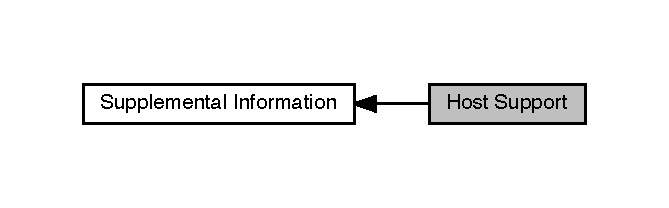
\includegraphics[width=321pt]{a00373}
\end{center}
\end{figure}
